\documentclass[conference]{IEEEtran}
\IEEEoverridecommandlockouts
% The preceding line is only needed to identify funding in the first footnote. If that is unneeded, please comment it out.
%Template version as of 6/27/2024

\usepackage{cite}
\usepackage{amsmath,amssymb,amsfonts}
\usepackage{algorithmic}
\usepackage{graphicx}
\usepackage{textcomp}
\usepackage{xcolor}
\usepackage{placeins}
\usepackage{float}

\def\BibTeX{{\rm B\kern-.05em{\sc i\kern-.025em b}\kern-.08em
    T\kern-.1667em\lower.7ex\hbox{E}\kern-.125emX}}
\begin{document}

\title{Signal Processing Front-Ends for EEG-Based Emotion and Mental-State Recognition: A Comprehensive Review}

\author{
    \IEEEauthorblockN{Edgie Bajuyo}
    \IEEEauthorblockA{
        \textit{Department of Computer Engineering} \\
        \textit{University of Science and Technology}\\ 
        \textit{of Southern Philippines} \\
        Cagayan de Oro City, Philippines \\
        bajuyo.edgieroszel21@gmail.com
    \and
    \IEEEauthorblockN{Adriane Loquinte}
    \IEEEauthorblockA{
        \textit{Department of Computer Engineering} \\
        \textit{University of Science and Technology}\\ 
        \textit{of Southern Philippines} \\
        Cagayan de Oro City, Philippines \\
        adrianeloquinte@gmail.com
    \and
    \IEEEauthorblockN{Uriel Dionsay}
    \IEEEauthorblockA{
        \textit{Department of Computer Engineering} \\
        \textit{University of Science and Technology}\\ 
        \textit{of Southern Philippines} \\
        Cagayan de Oro City, Philippines \\
       urieldionsay@gmail.com
}
}
}
}
\maketitle

\begin{abstract} 
This review surveys digital signal processing methods for electroencephalography-based emotion and mental-state recognition with machine learning. The paper organizes recent approaches into three practical patterns and a neuromorphic alternative: (1) time–frequency image pipelines that convert electroencephalography windows to continuous wavelet transform scalograms, extract convolutional features, and classify with a multiclass support vector machine; reported gains come from using early convolutional layers and subject-independent evaluation. (2) hybrid convolutional neural network–long short-term memory designs that apply standard preprocessing and feature formation (including entropy and band-power) before per-window convolution and across-window sequence modeling; these have achieved high accuracy on standard benchmarks. (3) feature-centric pipelines that either use entropy families (approximate, sample, permutation, differential, multiscale fuzzy, wavelet) with classical classifiers or learn multiple-feature-block convolutional representations for continuous decoding in operational settings. A neuromorphic route encodes engineered features such as discrete wavelet transform coefficients, fast Fourier transform magnitudes, and variance into spikes for spiking neural network classification.

Common challenges include inter-subject variability, noise and non-stationarity, heterogeneous pipelines that hinder comparability, computational cost of large backbones, and dataset inconsistencies. The paper outlines practical responses used across the reviewed studies: subject-independent protocols such as leave-one-subject-out cross-validation; consistent filtering, normalization, and fixed windowing; artifact handling with Independent Component Analysis when needed; preference for compact models or early-layer feature taps with lightweight classifiers; and harmonized preprocessing and label schemes for cross-dataset work. Overall, the review highlights reproducible digital signal processing choices and model designs that balance accuracy, efficiency, and deployment feasibility for electroencephalography-based emotion and mental-state recognition.
\end{abstract}

\begin{IEEEkeywords}
Electroencephalogram (EEG), Emotion Recognition, Digital Signal Processing (DSP), Machine Learning, Feature Extraction, Deep Learning, CNN, LSTM.
\end{IEEEkeywords}

\section{Introduction}
The analysis of Electroencephalogram (EEG) signals has emerged as a significant area of research, offering a non-invasive window into the complexities of human brain function. In recent years, emotion and mental state recognition from electroencephalography is an increasingly important direction in human–computer interaction, mental health assessment, and adaptive multimedia systems as it enables machine learning systems to infer internal cognitive–affective dynamics from noninvasive neural signals. 

There has been a considerable convergence of Digital Signal Processing (DSP) and Machine Learning (ML) to decode these signals for a variety of applications, Traditional pipelines have relied on band-limited preprocessing and handcrafted features, but their sensitivity to artifacts, subject variability, and non-stationarity often limits generalization across individuals and recording sessions \cite{Hag2021StressHybridFS_Sensors,Hamzah2024HeliyonEEGERSurvey}

 We are observing a clear trend where DSP-based feature extraction is not a separate preliminary step but is instead intricately woven into the architecture of advanced models. This includes the usage of Wavelet Convolutional Neural Network (WCNN) and Support Vector Machine (SVM) \cite{Bagherzadeh2023HybridEEGWaveletCNN_SVM} where it basically converts electroencephalography (EEG) windows into continuous wavelet transform scalograms. This approach also uses several references where it also makes use of explicit time–frequency images plus a convolutional neural network feature extractor and finishes with a classical margin-based classifier \cite{Hag2021StressHybridFS_Sensors,Hamzah2024HeliyonEEGERSurvey}. Similarly, \cite{Chakravarthi2022EEGHybridCNNLSTM} makes use of EEG Recognition through the usage of hybrid CNN and Long short-term Memory Classification (LSTM) which combines convolutional neural network with a long short-term memory module after standard preprocessing and feature formation, aligning with the hybrid convolutional neural network–recurrent neural network designs highlighted and contextualized in the deep-learning survey \cite{Jung2022VR_Emotion_IJERPH}.

 As of recent, there are numerous amounts of features for CNN that can coincide with the recognition of emotion and mental states. Such as that of \cite{Patel2021EEGEntropyReview, Lee2020MFB_CNN_PilotMentalStates} which focuses on the usage of entropy and other multiple features that can determine and decode a person's mental state. Specifically, the former \cite{Patel2021EEGEntropyReview} uses mathematically defined entropy descriptors as the primary digital signal processing representation and evaluates with standard supervised classifiers \cite{Hamzah2024HeliyonEEGERSurvey,Chen2025AdvancesEEGEmotion_ASOC}. Whereas, the latter \cite{Lee2020MFB_CNN_PilotMentalStates} uses a tailored convolutional neural network directly on electroencephalography (with minimal handcrafted features) and targets continuous, sliding-window inference rather than only trial-wise emotion labels \cite{Hag2021StressHybridFS_Sensors}.
 In a way, \cite{Luo2020SNN_EEGEmotion} is also an approach where it uses spiking neural networks and basically extracts engineered features per window which then converts them into spike trains. In itself, it's a rather distinct approach that keeps a conventional digital signal processing front-end but replaces standard classifiers with a spiking neural network to exploit spike-based computation \cite{Wang2023DL_EEG_Review}.

 Through these advances, this paper proposes the usage of several processing techniques that work alongside with the training of appropriate models. This review paper aims to introduce several approaches to realizing EGG-Recognition for both emotion and mental spectrum in order to be used alongside machine learning or basically the training of appropriate models.
\section{Methodology}
The intellectual challenge of decoding emotions from EEG signals lies not in a single algorithm, but in the thoughtful construction of a multi-stage processing pipeline. This section dissects this symbiotic relationship.

\subsection{Wavelet Convolutional Neural Networks and Support Vector Machine}
A pivotal insight in recent research is that the representation of data is as crucial as the classification model itself. One dominant trend is the transmutation of 1D EEG time-series data into 2D time-frequency representations, effectively turning a signal processing problem into a computer vision one. Time-frequency (TF) methods \cite{Pachori2023TimeFrequencyBook}, such as the Continuous Wavelet Transform (CWT), can convert a 1D EEG signal into a 2D representation that captures the spectral variation of the signal over time. One dimension corresponds to time while the other represents frequency, forming an image that reflects EEG power fluctuations across both domains. This process models the signal as a linear combination of basic functions known as wavelets, mathematically expressed as:

\begin{equation}
W_{(a,b)}[x(t)] = \frac{1}{|a|^{1/2}} \int_{-\infty}^{+\infty} x(t)\,\varphi^{*}\!\left(\frac{t - b}{a}\right) dt
\end{equation}

where \(a\) is the scale (a real and positive value), \(b\) is the translational parameter (a real number), and \(\varphi\) denotes the mother wavelet, which localizes the signal in both time and frequency domains.

This image representation of EEG power changes in time and frequency effectively captures the transient, non-stationary nature of neural oscillations. Similarly, \cite{Bagherzadeh2023HybridEEGWaveletCNN_SVM} provides a compelling demonstration of this, employing the CWT to generate scalograms. These 2D images allow researchers to leverage the immense power of pre-trained Convolutional Neural Networks (CNNs) \cite{Bagherzadeh2023HybridEEGWaveletCNN_SVM}. In the study, the deep features learned by a pre-trained ResNet-18 from the CWT scalograms were subsequently fed into a Multiclass Support Vector Machine (MSVM) \cite{Bagherzadeh2023HybridEEGWaveletCNN_SVM}. This hybrid strategy, which separates the task of feature representation from classification, significantly boosted performance on the MAHNOB-HCI dataset.

Four pre-trained CNNs were evaluated using three performance measures—accuracy, precision, and recall—through the leave-one-subject-out cross-validation (LOSO-CV) \cite{Pauli2021BalancedLOSO} approach. In this approach, data from 31 subjects were used to fine-tune existing CNNs, while data from another subject were used as the test set. This ensures subject independence, as no samples from a single subject appear in both the training and testing sets. The process repeats until all subjects have been tested once, and the final reported results are the mean and standard deviation across all iterations.

Accuracy, precision, and recall \cite{Powers2020EvaluationArXiv} are calculated as follows:

\begin{equation}
Accuracy = \frac{1}{l} \sum_{i=1}^{l} \frac{tp_i + tn_i}{tp_i + tn_i + fp_i + fn_i}
\end{equation}

\begin{equation}
Precision = \frac{1}{l} \sum_{i=1}^{l} \frac{tp_i}{tp_i + fp_i}
\end{equation}

\begin{equation}
Recall = \frac{1}{l} \sum_{i=1}^{l} \frac{tp_i}{tp_i + fn_i}
\end{equation}

where \(tp_i\), \(tn_i\), \(fp_i\), and \(fn_i\) denote the true positive, true negative, false positive, and false negative counts, respectively, for each emotional class derived from the confusion matrix of the classifier.


\subsection{Hybrid CNN and LSTM Classification}
Another powerful approach involves creating hybrid architectures that combine different neural network types to process EEG data. The CNN-LSTM architecture is a prime example, leveraging the spatial feature learning of CNNs with the temporal sequence modeling of LSTMs. \cite{Chakravarthi2022EEGHybridCNNLSTM} exemplifies this with a model that integrates a CNN, LSTM, and a ResNet-152 backbone \cite{Shanmugasundaram2024APLResNet152}.

\begin{figure}[H]
    \centering
    \includegraphics[width=\linewidth]{figures/eeg_flow_diagram.jpg}
    \caption{The flow of electroencephalography (EEG) data processing, showing sequential stages from raw EEG input, preprocessing, feature modeling, and emotion classification.}
    \label{fig:eeg_flow}
\end{figure}

The general EEG-based emotion identification process begins with data acquisition and preprocessing, as shown in Figure~\ref{fig:eeg_flow}. EEG data are collected and normalized to ensure consistency across sessions and subjects. Noise and artifacts are then mitigated using band-pass filters, typically in the range of 1–75 Hz, to preserve relevant frequency components. After preprocessing, the signals are transformed into structured representations such as Mel Frequency Cepstral Coefficients (MFCCs) \cite{Chakravarthi2022EEGHybridCNNLSTM}, entropy parameters, or topographic feature maps. These representations serve as the input to the hybrid CNN-LSTM network, which learns spatial features through convolutional layers and temporal dependencies through recurrent layers. This combined approach enhances the model’s ability to recognize emotion-related EEG patterns and classify them accurately.

\begin{figure}[H]
    \centering
    \includegraphics[width=0.8\linewidth]{figures/cnn_lstm_framework.jpg}
    \caption{Overview of the CNN-LSTM methodology, showing stages from preprocessing, feature extraction, model application, and performance evaluation.}
    \label{fig:cnn_lstm_framework}
\end{figure}

Figure~\ref{fig:cnn_lstm_framework} presents the complete methodological framework of the CNN-LSTM model used for EEG-based emotion classification. The model merges a homogeneous CNN and LSTM classifier with the ResNet-152 backbone to maximize both spatial and temporal feature representation. The SEED-V EEG dataset—comprising emotional states such as happiness, disgust, fear, neutral, and sadness—was used to evaluate this model. Preprocessing was conducted to prepare EEG data channels (FP1, FP2, FC6, and F3), followed by feature extraction through MFCC \cite{Chakravarthi2022EEGHybridCNNLSTM} computation and entropy analysis. The entropy was calculated using the sample entropy method, while the Hurst exponent was determined via R/S analysis to capture signal complexity and variability.

The extracted features were converted into topographic maps that served as CNN inputs, while the LSTM layers modeled the temporal dynamics of these representations. Both CNN and CNN-LSTM configurations employing ResNet-152 were trained and compared. The models classified emotional states and conditions such as PTSD and non-PTSD, with performance evaluated using standard metrics including accuracy, precision, recall, and F1-score. This end-to-end framework demonstrates the hybrid model’s capacity to fuse spatial-spectral and temporal information for robust EEG-based emotion recognition.


\subsection{Multiple Feature Block-Based Extraction Measure}
In EEG-based emotion and mental state recognition, one emerging approach focuses on enhancing feature representation by integrating domain knowledge directly into the network design. Rather than relying purely on end-to-end deep learning, these methods combine handcrafted feature engineering with specialized convolutional architectures. This strategy bridges the interpretability of traditional DSP-based features with the adaptability of deep neural models. The goal is to capture complex temporal and spatial patterns from EEG signals while preserving meaningful relationships within the data, leading to more reliable cognitive state recognition.

\begin{figure}[H]
    \centering
    \includegraphics[width=\linewidth]{figures/mfb_cnn_pipeline.png}
    \caption{Overview of the MFB-CNN workflow for EEG-based mental state classification, illustrating stages from EEG acquisition and preprocessing to temporal–spatial feature extraction and final classification into cognitive states.}
    \label{fig:mfb_cnn_pipeline}
\end{figure}

A particularly salient feature in this domain is entropy, which quantifies the signal’s complexity. \cite{Patel2021EEGEntropyReview} explored how various entropy-based measures—including Differential Entropy (DE), Sample Entropy (SampEn), and Approximate Entropy (ApEn) \cite{Patel2021EEGEntropyReview}—can serve as potent indicators of emotional states. These handcrafted features are then classified using traditional machine learning models such as SVM, k-NN, and Decision Trees.

Building upon this foundation, \cite{Lee2020MFB_CNN_PilotMentalStates} proposed the Multiple Feature Block-based Convolutional Neural Network (MFB-CNN), a hybrid model designed to decode mental states in high-interference environments such as simulated flight. Because EEG data in such settings are susceptible to motion artifacts, preprocessing plays a vital role. Artifacts were removed using Independent Component Analysis (ICA) \cite{Lee2020MFB_CNN_PilotMentalStates}, where four EOG channels were designated as contamination references. Signal processing and experimental control were implemented using MATLAB 2019a with the BBCI toolbox.

After preprocessing, the EEG dataset consisted of all recorded channels and sampling points (300 × 300) as input matrices. The MFB-CNN was structured into seven convolutional blocks organized hierarchically to enable progressive feature abstraction. Each convolutional block contained four convolutional layers and one batch-normalization layer with a filter size of 32. Temporal feature extraction used filter sizes of 1 × 5, while spatial feature extraction in later blocks used 3 × 1 filters to capture inter-channel dependencies. Dropout layers with a rate of 0.5 were applied to prevent overfitting, and max- and average-pooling layers reduced redundant information while retaining essential activation patterns.

An exponential linear unit (ELU) activation function was applied in the seventh convolutional block to improve nonlinear learning efficiency, defined as:

\begin{equation}
ELU(x) =
\begin{cases}
x, & \text{if } x > 0 \\
\alpha (e^{x} - 1), & \text{if } x \leq 0
\end{cases}
\end{equation}

For model training, the network was iteratively trained over 30 epochs, and classification accuracies were evaluated on the test data. The MFB-CNN successfully classified EEG patterns into cognitive states such as normal, distraction, fatigue, and workload, achieving an offline accuracy of 0.75. This result underscores the potential of the MFB-CNN framework to capture both temporal and spatial dependencies for real-time mental state monitoring.


\subsection{Spiking Neural Networks}
Venturing beyond conventional deep learning, some researchers are exploring neuromorphic approaches that emulate biological neural behavior more closely. Spiking Neural Networks (SNNs) \cite{Luo2020SNN_EEGEmotion} operate on event-driven computations, processing information as discrete spikes rather than continuous activations. This time-based mechanism enables SNNs to capture temporal dependencies within EEG signals efficiently while consuming significantly less power—making them ideal for real-time emotion recognition and wearable applications.

\begin{figure}[H]
    \centering
    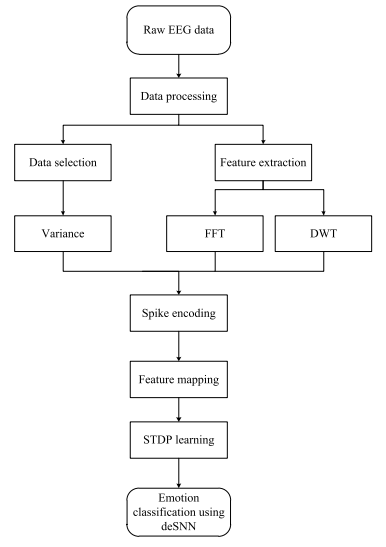
\includegraphics[width=0.7\linewidth]{figures/desnn_pipeline.png}
    \caption{Workflow of EEG signal processing and emotion classification using deSNN, showing the stages from raw EEG input through feature extraction, spike encoding, and STDP-based classification.}
    \label{fig:desnn_pipeline}
\end{figure}

As shown in Figure~\ref{fig:desnn_pipeline}, EEG-based emotion recognition using SNNs follows a structured pipeline: data processing, feature extraction, and classification. The raw EEG data undergo preprocessing to remove noise and artifacts. Datasets such as DEAP or SEED [15] are typically down-sampled to 128–200 Hz and filtered using a band-pass filter (0.75–45 Hz) via EEGLAB or similar toolboxes. Signals are separated into frequency bands (alpha, beta, gamma, and theta), corresponding to specific physiological and cognitive states.

Feature extraction then integrates both time-domain and frequency-domain analyses to generate spike-compatible features. In the time domain, the variance of EEG signals helps identify steady emotional states, computed as:

\begin{equation}
\mu_{\xi} = \frac{\xi(t_1) + \xi(t_2) + \dots + \xi(t_T)}{T}, \quad
v_{\xi} = \frac{1}{T} \sum_{t=1}^{T} [\xi(t) - \mu_{\xi}]^2
\end{equation}

In the frequency domain, the Fast Fourier Transform (FFT) and Discrete Wavelet Transform (DWT) \cite{Luo2020SNN_EEGEmotion} are applied to extract oscillatory and transient features. The DFT of the EEG signal \( \xi(t) \) is expressed as:

\begin{equation}
\xi(k) = DFT[\xi(t)] = \sum_{t=0}^{N-1} \xi(t) W_N^{tk}, \quad W_N^k = e^{-j \frac{2\pi k}{N}}
\end{equation}

and the maximum frequency measurable by the Nyquist theorem is \( f_{max} = \frac{f_s}{2} \), where \( f_s \) is the sampling frequency.  
For the DWT, non-stationary EEG signals are decomposed into multiple scales, providing localized frequency information. It is given by:

\begin{equation}
W(a,b) = \frac{1}{\sqrt{|a|}} \int s(t) \psi^* \left( \frac{t - b}{a} \right) dt
\end{equation}

where \(a\) and \(b\) represent the scaling and translation parameters, and \(\psi(t)\) is the mother wavelet, often the “db4” wavelet for EEG applications.

After these transformations, features are spike-encoded, converting continuous amplitude information into discrete spike trains. These spike patterns are then used as input to a spiking network, where temporal learning mechanisms such as Spike-Timing-Dependent Plasticity (STDP) \cite{Luo2020SNN_EEGEmotion} dynamically adjust synaptic weights according to spike timing differences.

\begin{figure}[H]
    \centering
    \includegraphics[width=0.7\linewidth]{figures/neucube_structure.png}
    \caption{Architecture of the NeuCube SNN framework showing the 3D spatio-temporal neuron cube and EEG electrode mappings used for encoding and classification.}
    \label{fig:neucube_structure}
\end{figure}

A well-known implementation of SNN for emotion classification is the NeuCube model, which employs a 3D spatio-temporal neural reservoir. As illustrated in Figure~\ref{fig:neucube_structure}, the NeuCube architecture is composed of three principal components: (1) an input module for temporal encoding, (2) the 3D SNNcube for dynamic mapping of EEG signals, and (3) an evolving SNN classifier. Temporal coding is employed to represent EEG data where the timing of spikes carries information about the signal amplitude and frequency characteristics.

The NeuCube typically consists of 1000 neurons arranged in a 10×10×10 lattice structure based on the small-world connectivity principle, which ensures efficient information transfer among neurons. The neurons are interconnected through proximity-based weights, forming both short-range and long-range connections that simulate biological cortical networks. During initialization, input neurons corresponding to EEG electrode sites (e.g., FP1, FP2, FC2, and O1) are mapped spatially to specific nodes in the SNNcube.

The learning process in NeuCube utilizes a variant of the STDP rule to modify synaptic weights between presynaptic and postsynaptic neurons depending on their firing intervals. The STDP weight update function is defined as:

\begin{equation}
\begin{aligned}
w_{ij}(t + 1) &= w_{ij}(t) + \Delta w_{ij}, \\
\Delta w_{ij} &=
\begin{cases}
A^+ e^{-\Delta t / \tau^+}, & \text{if } \Delta t > 0, \\
-A^- e^{\Delta t / \tau^-}, & \text{if } \Delta t \leq 0.
\end{cases}
\end{aligned}
\end{equation}

where \(\Delta t\) is the time difference between presynaptic and postsynaptic spikes, \(A^+\) and \(A^-\) are learning rate constants, and \(\tau^+\) and \(\tau^-\) are time constants for potentiation and depression, respectively. Positive \(\Delta t\) values increase synaptic strength (potentiation), while negative \(\Delta t\) values lead to depression.

Once trained, the NeuCube model classifies emotions by recognizing characteristic spatio-temporal spike patterns corresponding to different emotional states. This approach demonstrates how biologically inspired SNNs can bridge the gap between neuroscience and machine learning—achieving efficient, interpretable, and temporally precise emotion decoding from EEG signals.


\subsection{Comparative Analysis of Reviewed Studies}
To distill the diverse strategies into a coherent overview, this section presents a comparative analysis of the primary methodologies reviewed. Table \ref{tab:method_similarities} highlights the common threads and shared principles among the studies, while Table \ref{tab:summary_journal} provides a detailed summary of each paper.

\begin{table}[htbp]
\centering
\scriptsize
\caption{Comparative Analysis of Methodological Similarities}
\label{tab:method_similarities}
\renewcommand{\arraystretch}{2}
\begin{tabular}{p{1.5cm}p{2.5cm}p{4cm}}
\hline
\textbf{Ref.} & \textbf{Approach} & \textbf{Similarities} \\
\hline
\textbf{\cite{Bagherzadeh2023HybridEEGWaveletCNN_SVM}}
& Wavelet Convolutional Neural Networks and Support Vector Machine
& The usage of wavelet convolutional neural networks along with support vector machines plays a fairly crucial role in this study as it provides a way to convert electroencephalography windows into continuous wavelet transform scalograms, which is proven necessary for further research due to the usage of convolutional neural networks \\[1mm]
\textbf{\cite{Chakravarthi2022EEGHybridCNNLSTM}}
& Hybrid Convolutional Neural Network and Long Short-term Memory Classification
& Hybrid convolutional neural network and long short-term memory classification basically implements hybrid models (CNN+LSTM) to capitalize on the strengths of two-stage deep architecture that separates per-window representation from across-window dynamics. \\[1mm]
\textbf{\cite{Patel2021EEGEntropyReview}}
& Entropy as a Feature Extraction Measure
& Entropy as a feature extraction measure uses mathematically defined entropy descriptors as the primary digital signal processing representation and evaluates with standard supervised classifiers. This works similarly with other features for convolutional neural network\\[1mm]
\textbf{\cite{Lee2020MFB_CNN_PilotMentalStates}}
& Multiple Feature Block-Based Convolutional Neural Network
& Block-based convolutional neural network features multiple Uses that are tailored to convolutional neural network which operates directly on electroencephalography and targets continuous, sliding-window inference rather than only trial-wise emotion labels. \\[1mm]
\textbf{\cite{Luo2020SNN_EEGEmotion}}
& Usage of Spiking Neural Networks
& Spiking neural networks uses a distinct approach that keeps a conventional digital signal processing front-end but replaces standard classifiers with a spiking neural network to exploit spike-based computation. \\[1mm]
\hline
\end{tabular}
\end{table}
\FloatBarrier
The analysis across these studies reveals several key trends. As highlighted in Table \ref{tab:method_similarities}, The goal is to show, at a glance, which methods belong to the same family so that later comparisons are fair. This table also basically finds similarities between these main references in order to state the common idea these pipelines share (for example, time–frequency image formation, sequence modeling across windows, use of mathematically defined features, sliding-window inference, or engineered features with a nonstandard classifier). This table is present to justify why the paper groups methods the way it does, and to make the evaluation choices (preprocessing, windowing, feature formation, classifier) transparent and comparable across studies.

\begin{table}[htbp]
    \caption{Summary of Reviewed Journal Papers}
    \centering
    \renewcommand{\arraystretch}{2}
    \large
    \resizebox{\columnwidth}{!}{
    \begin{tabular}{p{3cm} p{2.5cm} p{5cm} p{4cm}} 
        \hline
        \textbf{Paper Title} & \textbf{Focus} & \textbf{Mathematical Tools Used} & \textbf{Key Findings} \\
        \hline
        A Hybrid EEG-Based Emotion Recognition Approach Using Wavelet Convolutional Neural Networks and Support Vector Machine \cite{Bagherzadeh2023HybridEEGWaveletCNN_SVM}
        & Conversion of electroencephalography windows to time–frequency images and classify emotions with deep features plus a classical classifier.
        & Continuous Wavelet Transform to create scalograms; convolutional neural network intermediate feature maps; multiclass Support Vector Machine; leave-one-subject-out cross-validation.
        & Early-layer convolutional features combined with a multiclass Support Vector Machine improved accuracy versus end-to-end baselines; best results reported around 87.45\% (DEAP) on the Database for Emotion Analysis using Physiological Signals. \\
        
        EEG-based emotion recognition using hybrid CNN and LSTM networks \cite{Chakravarthi2022EEGHybridCNNLSTM}
        & Hybrid deep model that encodes per-window patterns and then models window-to-window evolution for emotion recognition.
        & Band-pass filtering and normalization; entropy measures such as sample entropy; band-power features in canonical frequency bands; convolutional neural network; long short-term memory recurrent module; softmax classification.
        & Reported accuracy of approximately 98\% on the Shanghai Jiao Tong University five-class dataset, outperforming support vector machine and artificial neural network baselines provided by the authors. \\
        
        EEG-based human emotion recognition using entropy as a feature extraction measure \cite{Patel2021EEGEntropyReview}
        & Survey and analysis of entropy-family features for emotion recognition from electroencephalography.
        & Approximate entropy; sample entropy; permutation entropy; differential entropy; multiscale fuzzy entropy; wavelet entropy; empirical mode decomposition–based entropies; classifiers such as support vector machines and k-nearest neighbors.
        & Shows that entropy features are effective descriptors of nonlinear dynamics; summarizes multiple studies with competitive results on common datasets, and positions entropy features as strong baselines and as inputs to modern models. \\
        
        Continuous EEG Decoding of Pilots’ Mental States Using Multiple Feature Block-Based Convolutional Neural Network \cite{Lee2020MFB_CNN_PilotMentalStates}
        & Continuous decoding of mental states such as fatigue, workload, and distraction using a tailored convolutional architecture.
        & Multiple feature block–based convolutional neural network with temporal and spatial filtering; sliding-window inference; cross-subject validation protocols.
        & Offline accuracy reported around 0.75\% with standard deviation near 0.04\%; pseudo-online detection around 0.72\% for fatigue and workload and around 0.61\% for distraction, demonstrating feasibility for continuous monitoring. \\
        
        EEG-Based Emotion Classification Using Spiking Neural Networks \cite{Luo2020SNN_EEGEmotion}
        & Neuromorphic classification of emotions using spike-encoded engineered features.
        & Discrete Wavelet Transform; Fast Fourier Transform; time-domain variance; spike encoding; spiking neural network classifier.
        & On the Database for Emotion Analysis using Physiological Signals, accuracies per affective dimension reported around 74\% to 86\%. \\
        \hline
    \end{tabular}
    }
    \label{tab:summary_journal}
\end{table}

\FloatBarrier 

Table \ref{tab:summary_journal} presents a comparative summary of five journal papers, each addressing key challenges in electroencephalography-based emotion and mental-state recognition. Although the problem settings differ (trial-wise emotion classification versus continuous state decoding), the papers collectively advance practical digital signal processing pipelines for analyzing electroencephalography data.

Despite using different mathematical tools—ranging from time–frequency analysis with continuous wavelet transform and convolutional feature extraction, to hybrid convolutional neural network–long short-term memory models, entropy-based feature sets with classical classifiers, multiple-feature-block convolutional networks for continuous decoding, and spiking neural networks with engineered features—the studies share a common objective: improving accuracy and robustness under subject-wise evaluation while keeping computation feasible for deployment. 

These shared methodologies underline the broader significance of structured preprocessing, well-defined feature construction, and clearly stated evaluation protocols in building reliable, reproducible electroencephalography emotion recognition systems.


\section{Challenges and Issues}
Challenges arise at multiple stages in developing and implementing EEG-based emotion recognition systems. One major challenge lies in managing the high inter-subject variability of EEG signals. Neural patterns associated with identical emotional states differ significantly across individuals, leading to inconsistencies in model generalization. To address this, studies such as the CWT-CNN approach \cite{Bagherzadeh2023HybridEEGWaveletCNN_SVM} employ Leave-One-Subject-Out Cross-Validation (LOSO-CV) to evaluate inter-person robustness. Achieving consistent accuracy across subjects remains difficult due to variations in electrode placement, signal amplitude, and noise characteristics inherent to EEG recordings.

The noise-prone and non-stationary nature of EEG data also presents a considerable obstacle. Motion artifacts, muscle activity, and environmental interference often distort the signal, reducing its discriminative power. The MFB-CNN model \cite{Lee2020MFB_CNN_PilotMentalStates}, implemented in a simulated flight environment, required extensive preprocessing using Independent Component Analysis (ICA) to remove motion artifacts and eye-blink interference. Although such preprocessing improves signal quality, it significantly increases computational cost and limits real-time applicability.

Another persistent issue concerns the lack of methodological standardization across studies. Different research groups employ heterogeneous pipelines—ranging from CWT-CNN-SVM hybrids \cite{Bagherzadeh2023HybridEEGWaveletCNN_SVM} and CNN-LSTM frameworks \cite{Chakravarthi2022EEGHybridCNNLSTM} to MFB-CNN architectures \cite{Lee2020MFB_CNN_PilotMentalStates} and neuromorphic SNN models \cite{Luo2020SNN_EEGEmotion}. Each approach uses distinct preprocessing protocols, feature extraction strategies, and evaluation metrics, complicating the comparison of results across studies. This fragmentation hinders the establishment of consistent benchmarks and slows the development of reproducible EEG-based emotion recognition systems.

The computational complexity of deep learning models presents another difficulty. Architectures employing large backbones such as ResNet-152 \cite{Chakravarthi2022EEGHybridCNNLSTM} provide high accuracy but demand substantial computational resources for both training and inference. This constraint poses limitations for deployment in portable or embedded devices intended for continuous emotion monitoring. Spiking Neural Networks (SNNs) \cite{Luo2020SNN_EEGEmotion} have emerged as an energy-efficient alternative, yet they currently involve trade-offs between efficiency and precision, creating challenges in maintaining accuracy under low-power operation.

The scarcity and inconsistency of EEG datasets further constrain progress. Existing datasets differ in sampling rates, channel configurations, and labeling conventions, making cross-dataset evaluation and model transferability difficult. Data collection is resource-intensive and sensitive to subject-specific conditions, which restricts the availability of large, standardized datasets for robust training. Addressing these issues requires coordinated standardization of acquisition protocols, optimized preprocessing pipelines, and the design of computationally efficient models capable of operating under real-world variability.


\section{Solution}
To address high inter-subject variability and improve generalization across individuals, use subject-independent evaluation by default and report Leave-One-Subject-Out Cross-Validation, as done in the continuous wavelet transform plus convolutional neural network plus support vector machine study \cite{Bagherzadeh2023HybridEEGWaveletCNN_SVM}. Stabilize inputs with per-recording normalization and fixed, overlapping windowing before feature construction. When a simple baseline is needed, include entropy-based features that depend on distributional properties rather than absolute amplitudes to reduce sensitivity to subject scale differences \cite{Patel2021EEGEntropyReview}. For time–frequency image pipelines, aggregate channels into consistent regional groupings and use early convolutional features with a lightweight classifier, which showed better cross-subject behavior than deeper end-to-end settings in \cite{Bagherzadeh2023HybridEEGWaveletCNN_SVM}.

To reduce the impact of noise and non-stationarity, keep a short, repeatable preprocessing chain: task-appropriate band-pass, mains notch, fixed segmentation, and artifact removal when present. Independent Component Analysis should be applied when ocular or motion artifacts are visible; it was necessary for reliable operation in the multiple feature block–based convolutional neural network pilot study \cite{Lee2020MFB_CNN_PilotMentalStates}. For feature formation, use continuous wavelet transform scalograms to capture transient content for image-based models \cite{Bagherzadeh2023HybridEEGWaveletCNN_SVM} and entropy measures such as sample entropy, permutation entropy, and differential entropy to summarize irregularity in engineered-feature pipelines \cite{Patel2021EEGEntropyReview}.

To limit methodological fragmentation and make results comparable, lock a single protocol and report it completely: channel montage and reference, sampling rate, exact filter bands and notch frequency, window length and hop, whether Independent Component Analysis was used, the precise wavelet family and scales for continuous wavelet transform, and the exact definitions and parameters for each entropy measure. State clearly whether results are within-subject or cross-subject, and match the evaluation style of the main pipelines you are citing (for example, LOSO for \cite{Bagherzadeh2023HybridEEGWaveletCNN_SVM} and \cite{Lee2020MFB_CNN_PilotMentalStates}, sequence evaluation for \cite{Chakravarthi2022EEGHybridCNNLSTM}).

To manage computational complexity, replace very large backbones with compact alternatives or tap early convolutional layers and classify with a lightweight model. The wavelet plus convolutional neural network plus support vector machine pipeline in \cite{Bagherzadeh2023HybridEEGWaveletCNN_SVM} showed that early-layer features with a multiclass support vector machine can outperform deeper end-to-end models while reducing training and inference cost. In the convolutional neural network plus long short-term memory setting \cite{Chakravarthi2022EEGHybridCNNLSTM}, keep the convolutional front-end and the recurrent depth minimal and limit input resolution and sequence length to what is needed for accuracy. For low-power targets, use engineered features such as discrete wavelet transform, fast Fourier transform, and time-domain variance with a spiking neural network; the neuromorphic approach in \cite{Luo2020SNN_EEGEmotion} reached competitive accuracy with a lower compute budget than conventional deep models.

To work around dataset scarcity and inconsistency, choose one primary dataset for all headline comparisons and resample any secondary datasets to a common sampling rate with a consistent reference montage before training. Map labels to a common scheme when definitions differ. Increase effective data volume using overlapping windows and balanced sampling across classes; these practices are standard in the hybrid pipelines of \cite{Bagherzadeh2023HybridEEGWaveletCNN_SVM,Chakravarthi2022EEGHybridCNNLSTM}. For continuous monitoring scenarios, keep the same sliding-window and pseudo-online evaluation used during development so that deployment conditions match validation, as in \cite{Lee2020MFB_CNN_PilotMentalStates}.
\section{Conclusion}
This review has synthesized the prevailing methodologies, challenges, and solutions in the field of EEG-based emotion recognition, based on literature published between 2022 and 2025. The findings show a clear and consistent trend: the deep integration of advanced DSP techniques with powerful machine learning models. The most successful approaches, such as transforming 1D EEG signals into 2D time-frequency representations for CNN analysis or using hybrid CNN-LSTM architectures to capture spatio-temporal dynamics, have become central to modern research and are pushing the boundaries of classification accuracy.

Despite the success of these methods, significant and persistent challenges impede the transition of these systems from controlled laboratory environments to practical, real-world applications. Key issues include the scarcity of large, high-quality datasets, the high degree of inter-subject variability in EEG signals, the lack of standardization in research protocols, and the computational expense of state-of-the-art models. These are not trivial problems, and they collectively hinder the development of robust, generalizable, and accessible emotion recognition technology.

In response, the research community is pursuing a multi-pronged strategy. To combat data limitations, data augmentation and synthesis using GANs are becoming mainstream. To address variability, transfer learning and domain adaptation techniques are being refined to create subject-independent models. For real-world deployment, there is a strong push towards developing lightweight, computationally efficient models suitable for resource-constrained devices. Finally, multimodal fusion, combining EEG with other physiological and behavioral data, is emerging as a key strategy for enhancing reliability.

In essence, the field is in a dynamic cycle of innovation where the solutions to today\'s challenges—such as data synthesis and model optimization—will form the core of tomorrow\'s more advanced methodologies. The convergence of sophisticated DSP and hybrid machine learning models represents the current frontier, paving the way for the next generation of systems that can reliably and ethically interpret human emotional states in real-time.


\bibliographystyle{IEEEtran}
\bibliography{BajuyoLoquinteDionsay_Lit_Rev_Ref}


\end{document}